\section{Collective I/O in ROMIO}
\label{sec: collio}
ROMIO is a popular implementation of the MPI-IO specification developed at the Argonne National Laboratory and currently supported by MPICH as well as OpenMPI and other packages. ROMIO provides parallel I/O functionalities for different file systems through the Abstract Device I/O interface~\cite{ThakurGL96} (ADIO). Latest versions of ROMIO include support for Lustre~\cite{Ying08}, GPFS~\cite{ProstTHKW00}, PVFS~\cite{CarnsLRT} and others through a dedicated ADIO driver.

\subsection{Two Phase I/O}
\label{sec: ext2ph}
In ROMIO, the core component of collective I/O is the `two phase I/O', also known as `extended two phase algorithm' (ext2ph)~\cite{ThakurC96}. The ROMIO implementation for collective I/O consists of several steps as follows:
\begin{figure}[!htb]
  \centering
  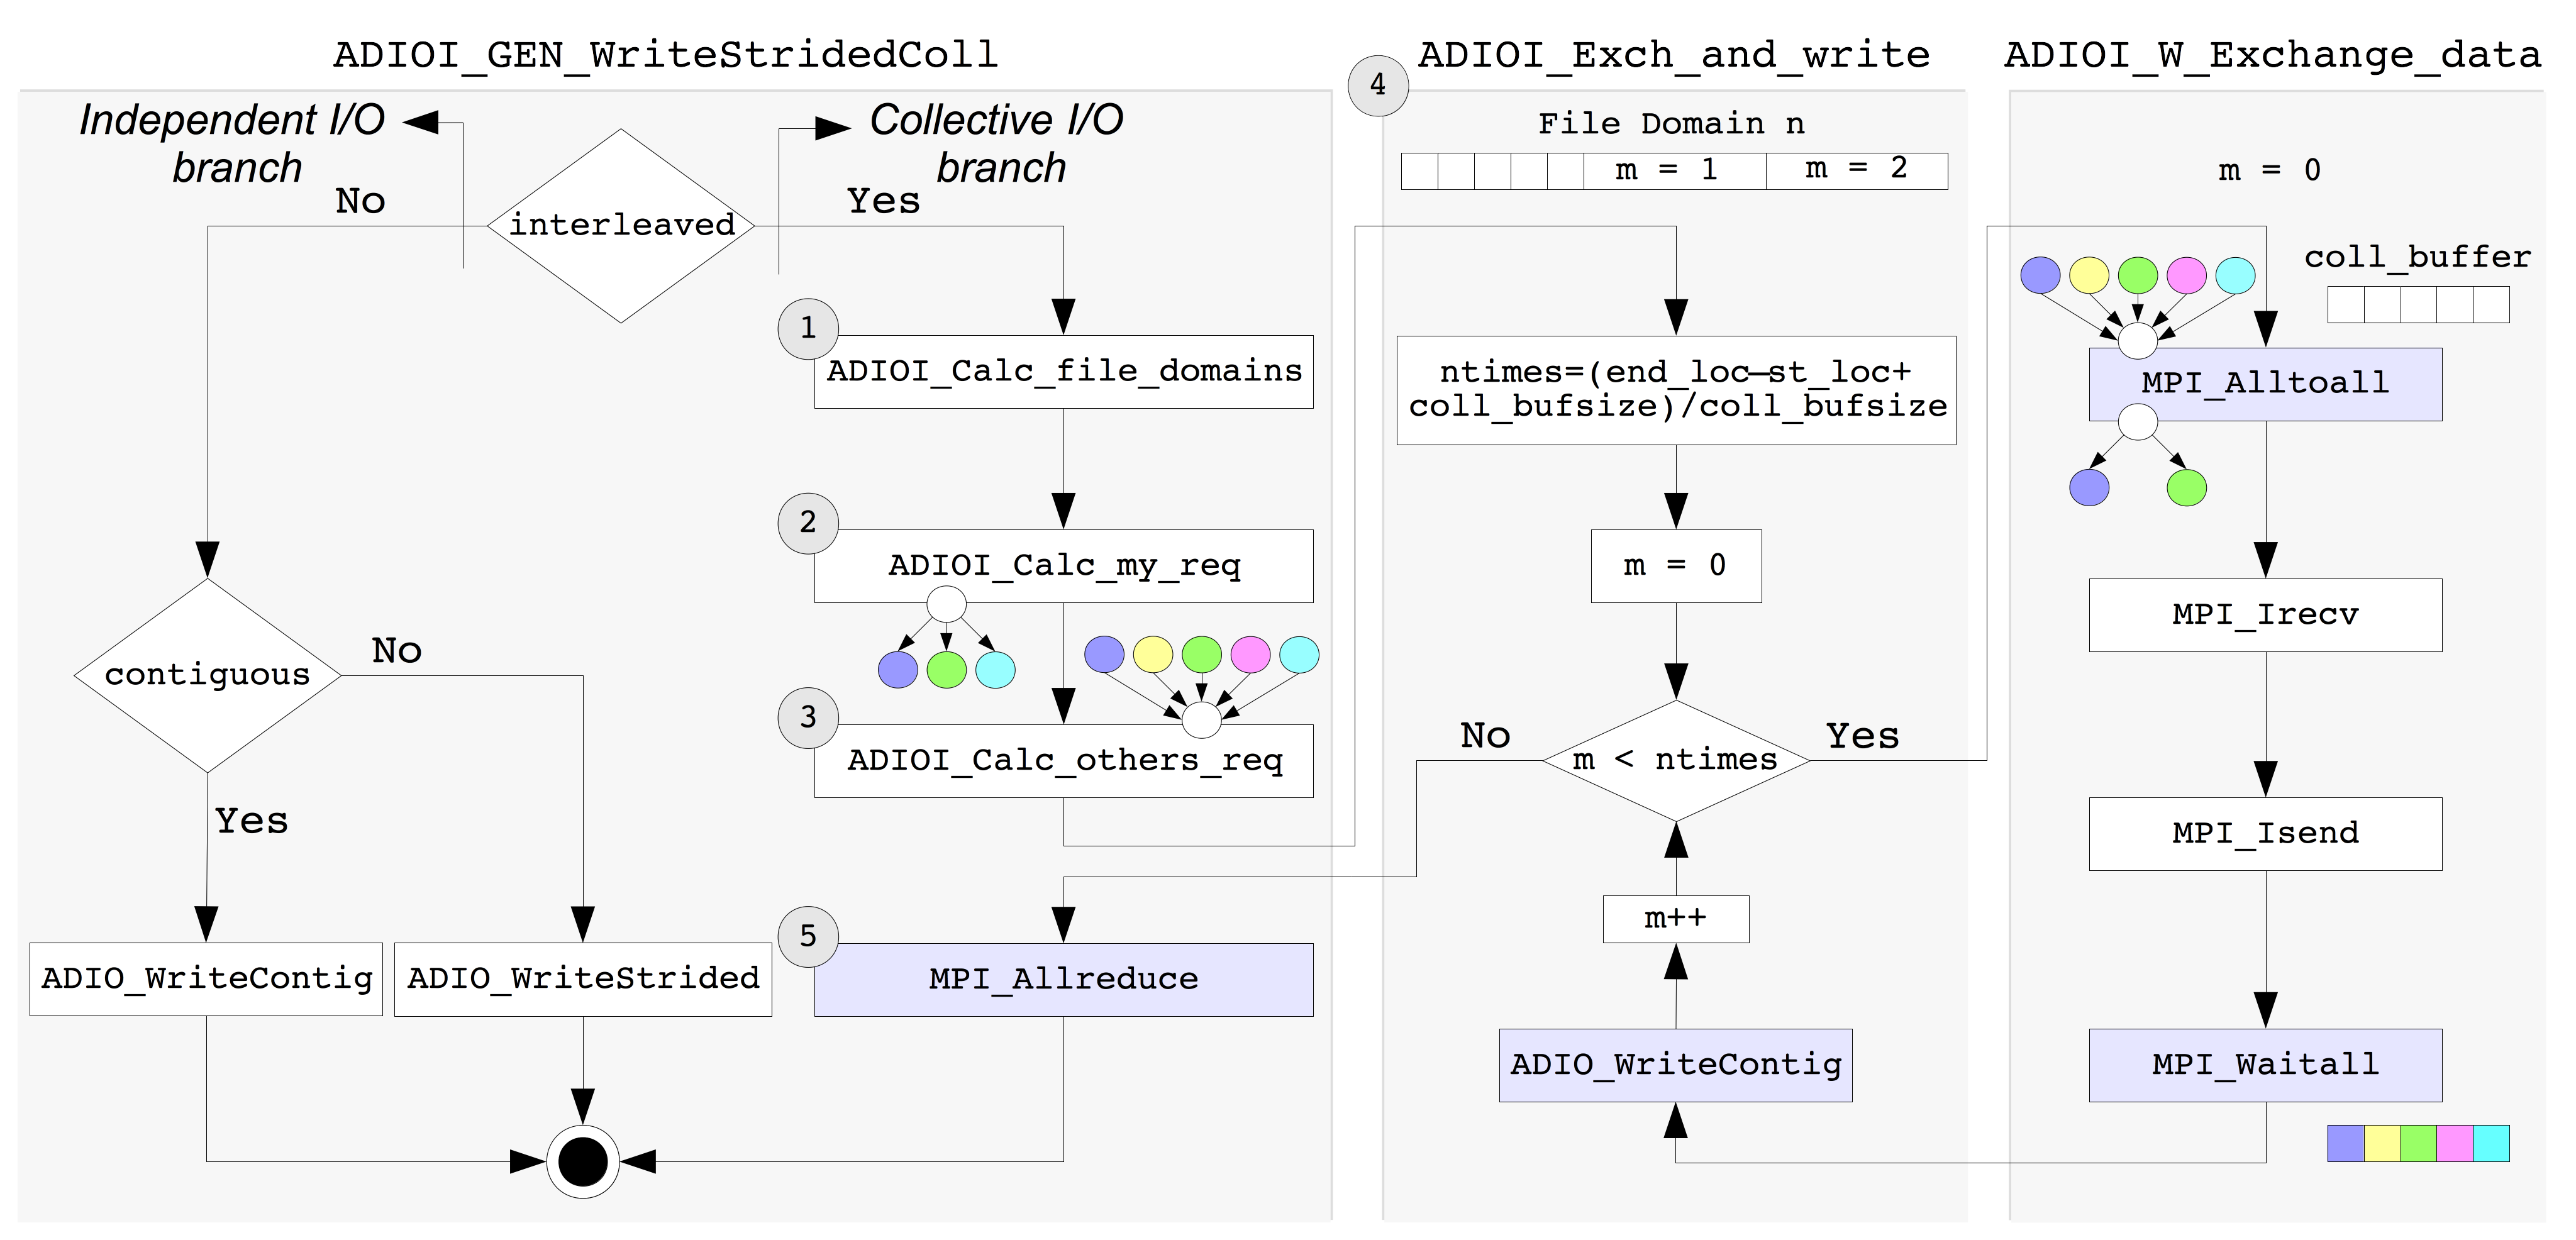
\includegraphics[width=\textwidth]{chapters/chapter3/figures/ext2ph}
  \caption{Collective I/O flow diagram for the write path in aggregators (non-aggregators neither receive nor write any data, just send it to aggregators). \codeword{MPI\_File\_write\_all()} invokes \codeword{ADIOI\_GEN\_WriteStridedColl()}. \codeword{ADIO\_WriteContig} is a macro that is replaced by \codeword{ADIOI\_GEN\_WriteContig()}. Performance critical functions for the collective I/O branch are highlighted in grey.}
  \label{figure: coll_io_impl}
\end{figure}

\begin{enumerate}
\item All processes taking part in the I/O operation exchange access pattern information with each other. The access pattern information is represented by start and end offsets for the accessed region (disregarding holes that may be present). Once file offsets are available, every process works out how big the global accessed region in the file is by taking maximum and minimum among all. The resulting byte range is divided by the number of available aggregators to build the so called `file domains' (contiguous byte ranges accessed independently by every aggregator).
\item Every process works out which file domains (and thus aggregators) its local data belongs to. In doing so, every process knows which aggregators it has to send (receive) data to (from), if any.
\item Every aggregator works out which other processes' requests map to its file domain. Doing so every aggregator knows what processes need to receive (in case of reads) or send (in case of writes) data for that particular file domain.
\item Actual two phase I/O starts. In the case of writes, that we exclusively consider here (the read case is similar), every process sends its data to the right aggregators (data shuffle phase) while these write the data to the parallel file system (data I/O phase). Data is written in blocks of predefined size (collective buffer size). If the size of the collective buffer is smaller than the file domain, the file domain is broken down into multiple sub-domains which are written in different rounds of the ext2ph algorithm. In order to handle multiple rounds of data shuffle and I/O, additional access information is required. This is disseminated by every process (collectively) to aggregators at the beginning of the data shuffle phase.
\item Once all the data has been written, all the processes must synchronise and exchange error codes. This is necessary to guarantee that it is safe to free the memory buffers containing the data.
\end{enumerate}
Figure~\ref{figure: coll_io_impl} shows how the previous steps map to the collective I/O implementation for the write operation. The collective write function (\codeword{MPI\_File\_write\_all()}) in ADIO is implemented through \codeword{ADIOI\_GEN\_WriteStridedColl()}. This is responsible for selecting the most suitable I/O method between those available. For example, independent I/O is selected if the access requests are not interleaved. Nevertheless, users can always enforce collective I/O by setting the appropriate MPI-IO hint. The \codeword{ADIOI\_Exch\_and\_write()} function contains the ext2ph algorithm implementation, including data shuffle and write methods. At the beginning of the data shuffle (\codeword{ADIOI\_W\_Exchange\_data()}) we have the dissemination function (\codeword{MPI\_Alltoall()}) used to exchange information concerning which part of the data has to be sent during a particular round of two phase I/O. 

There are three main contributors to collective I/O performance: (\textbf{a}) global synchronisation cost; (\textbf{b}) communication cost; and (\textbf{c}) write cost. \codeword{MPI\_Allreduce()} and \codeword{MPI\_Alltoall()} account for the global synchronisation cost. When a process reaches them it has to wait for all the other processes to arrive before continuing. \codeword{MPI\_Waitall()} accounts for communication cost since every process first issues all the non-blocking receives (if any) and sends, and afterwards waits for them to complete (refer to the right part of the diagram in Figure~\ref{figure: coll_io_impl}). Finally, \codeword{ADIO\_WriteContig()} accounts for write cost.

\subsection{Collective I/O Hints}
\label{subsec: hints}

Collective I/O behaviour can be controlled by users through a set of MPI-IO hints. Users can control whether collective I/O should be enabled or disabled with \codeword{romio\_cb\_write} and \codeword{romio\_cb\_read}, for write and read operations respectively, how many aggregators should be used during a collective I/O operation with \codeword{cb\_nodes} and how big the collective buffer should be with \codeword{cb\_buffer\_size}. Table~\ref{table: coll_io_hints_table} summarises the hints just described.

\begin{table}[!htb]
\centering
\ra{1.5}
\caption{Collective I/O hints in ROMIO.}
\newcolumntype{K}{>{\centering\arraybackslash} m{3cm}}
\newcolumntype{V}{>{\centering\arraybackslash} m{5.5cm}}
\begin{tabular}{KV}
\toprule
\bf \small Hint & \bf \small Description \\
\midrule
\small \codeword{romio\_cb\_write} & \small \codeword{enable} or \codeword{disable} collective writes \\
\small \codeword{romio\_cb\_read} & \small \codeword{enable} or \codeword{disable} collective reads \\
\small \codeword{cb\_buffer\_size} & \small set the collective buffer size [bytes]\\
\small \codeword{cb\_nodes} & \small set the number of aggregator processes\\
\bottomrule
\end{tabular}
\label{table: coll_io_hints_table}
\end{table}

Each of these hints has an effect on collective I/O performance. For example, by increasing the number of aggregators there will be a higher number of nodes writing to the parallel file system and thus a higher chance that one of these will experience variable performance due to load imbalance among available I/O servers, with increasing write time variation and associated global synchronisation cost. Furthermore, by increasing the collective buffer size users can reduce the number of two phase I/O rounds and, consequently, the number of global synchronisation events. Bigger collective buffers will also affect the write cost since more I/O servers will be accessed in parallel potentially increasing the aggregated I/O bandwidth.

Besides the hints described in Table~\ref{table: coll_io_hints_table}, there are other hints that do not directly concern collective I/O but affects its performance. The first is the \codeword{striping\_factor} hint, which defines how many I/O targets will be used to store the file. The second is the \codeword{striping\_unit} hint, which defines how big the data chunks written to each I/O target will be (in bytes). These two hints change the file characteristics in the parallel file system and typically the `striping\_unit' also defines the locking granularity for the file (e.g. Lustre).
